\section{图像重建}\label{sec:图像重建}
有了精心选好的图像样本后,我们需要把样本及其算出的辐射值
转化为用于显式或存储的像素值。根据信号处理理论,
我们需要做三件事来为输出图像中的每个像素计算最终值:
\begin{enumerate}
    \item 从图像样本集中重建连续的图像函数$\tilde{L}$.
    \item 对函数$\tilde{L}$预滤波以移除任何超过像素间隔对应的奈奎斯特上限的频率。
    \item 在像素位置采样$\tilde{L}$以计算最终像素值。
\end{enumerate}

因为我们知道我们将只在像素位置处重采样函数$\tilde{L}$,
所以没有必要构建该函数的显式表示。
相反,我们可以用单个滤波函数把前两步结合起来。

回想如果已经用大于奈奎斯特频率的频率对原始函数进行均匀采样
并用sinc滤波器重建,则第一步中的重建函数会完美匹配原始图像函数——
这是个壮举,毕竟我们只有样本点。
但因为图像函数几乎总是有比采样率所能处理的还高的频率(由边缘等造成),
我们选择对其不均匀地采样,把混叠换成噪声。

理想重建背后的理论依赖于均匀间隔的样本。
尽管已有大量将该理论拓展到非均匀采样的尝试,
但目前该问题还没有公认的解决方法。
此外,因为知道采样率不足以刻画函数,所以完美重建是不可能的。
采样理论领域最近的研究重新看待了重建问题,
明确承认实践中完美重建通常是不可能的。
这一观点的微笑转变带来了强大的重建新技术。
例如参见\citet{843002}了解关于这些进展的调研。
特别地,重建理论的研究目标已经从完美重建转为
开发能被证明可最小化重建函数与原始函数间差异的重建技术,
\emph{而不管原始函数是否是带限的}。

尽管pbrt中用的重建技术不是直接建立在这些新方法上的,
但它们能解释实践者的经验,即对图像合成所取的样本应用
完美重建技术通常不会得到最高质量的图像。
\begin{figure}[htbp]
    \centering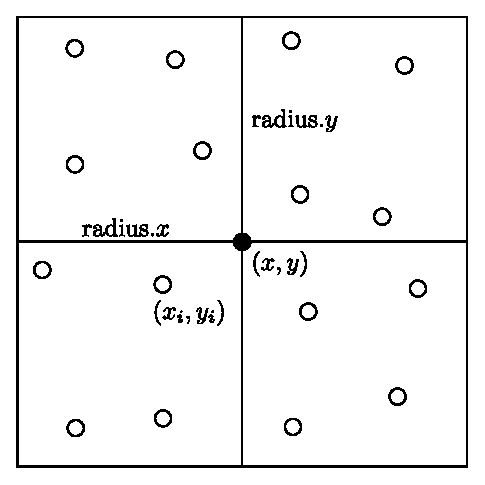
\includegraphics[width=0.5\linewidth]{chap07/2dimagefiltering.eps}
    \caption{2D图像滤波。为了给位于$(x,y)$处标为实心圆的像素
    计算滤波后的像素值,要考虑在$(x,y)$周围范围{\ttfamily radius.x}和
    {\ttfamily radius.y}以内方盒中的所有图像样本。
    每个表示为空心圆的图像样本$(x_i,y_i)$,都被2D滤波函数$f(x-x_i,y-y_i)$赋权。
    所有样本的加权平均即是最终的像素值。}
    \label{fig:7.38}
\end{figure}

为了重建像素值,我们将考虑在一特定像素旁对样本插值的问题。
为了给像素$I(x,y)$计算最终值,插值结果是计算加权平均
\begin{align}\label{eq:7.12}
    I(x,y)=\frac{\sum\limits_i {f(x-x_i,y-y_i)w(x_i,y_i)L(x_i,y_i)}}{\sum\limits_i {f(x-x_i,y-y_i)}}\, ,
\end{align}
其中
\begin{itemize}
    \item $L(x_i,y_i)$是位于$(x_i,y_i)$的第$i$个样本的辐亮度值;
    \item $w(x_i,y_i)$是\refvar{Camera}{}返回的样本贡献权重。
          如\refsub{相机测量方程}和\refsub{采样相机1}所述,
          计算这些权重的方法决定了胶片度量哪个辐射度学量。
    \item $f$是滤波函数。
\end{itemize}

\reffig{7.38}展示了位于$(x,y)$的像素,它有个在$x$和$y$方向
范围分别为{\ttfamily radius.x}和{\ttfamily radius.y}的像素滤波器。
在滤波器范围范围给出的方盒内的所有样本都可能对该像素值有贡献,
这取决于滤波函数值$f(x-x_i,y-y_i)$.

这里sinc滤波器不是合适的选择:回想当基本函数有超过奈奎斯特上限的频率时
理想sinc滤波器容易振铃(吉布斯现象),这意味着图像中的边缘在附近像素处
有微弱重复的边缘副本。此外,sinc滤波器有\emph{无限支撑}:
距离其中心的有限距离内它不会衰减到零,
所以对于每个输出像素都会需要滤波所有图像样本。实践中没有唯一最好的滤波函数。
为特定场景选择最好的需要结合定量评估与定性判断。

\subsection{滤波函数}\label{sub:滤波函数}
pbrt中的所有滤波器实现都从抽象类\refvar{Filter}{}派生,
它为滤波中用的函数$f(x,y)$提供了接口;见\refeq{7.12}。
(\refsec{胶片与成像管道}描述的)类\refvar{Film}{}存有指向\refvar{Filter}{}的指针
并在把图像样本的贡献累加到最终图像时对其滤波。
(\reffig{7.39}展示比较了用本节各种滤波器来重建像素值而渲染出的图像放大区域。)
基类\refvar{Filter}{}定义在文件\href{https://github.com/mmp/pbrt-v3/blob/master/src/core/filter.h}{\ttfamily core/filter.h}
和\href{https://github.com/mmp/pbrt-v3/blob/master/src/core/filter.cpp}{\ttfamily filter.cpp}中。
\begin{figure}[htbp]
    \centering
    \subfloat[矩形滤波器]{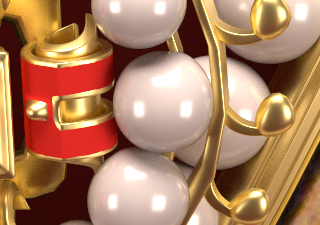
\includegraphics[width=0.62\linewidth]{chap07/crown-box.png}\label{fig:7.39.1}}\\
    \subfloat[高斯滤波器]{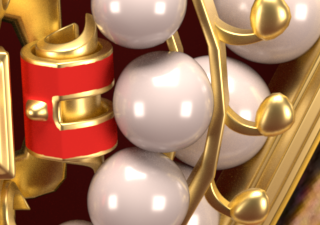
\includegraphics[width=0.62\linewidth]{chap07/crown-gaussian.png}\label{fig:7.39.2}}\\
    \subfloat[Mitchell-Netravali滤波器]{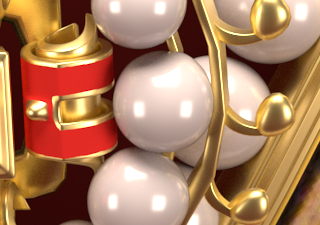
\includegraphics[width=0.62\linewidth]{chap07/crown-mitchell.png}\label{fig:7.39.3}}\\
    \caption{用来将图像样本转化为像素值的像素重建滤波器对最终图像的质量有明显的影响。
        这里我们看到用(a)矩形滤波器、(b)高斯以及(c) Mitchell-Netravali滤波器滤波的皇冠模型放大区域。
        注意Mitchell滤波器给出了最清晰的图像,而高斯则模糊了它。
        矩形是最不可取的,因为它允许高频混叠掺入到最终图像中
        (例如注意沿明亮金色边缘的阶梯状模式)。}
    \label{fig:7.39}
\end{figure}

\begin{lstlisting}
`\initcode{Filter Declarations}{=}`
class `\initvar{Filter}{}` {
public:
    `\refcode{Filter Interface}{}`
    `\refcode{Filter Public Data}{}`
};
\end{lstlisting}

\begin{figure}[htbp]
    \centering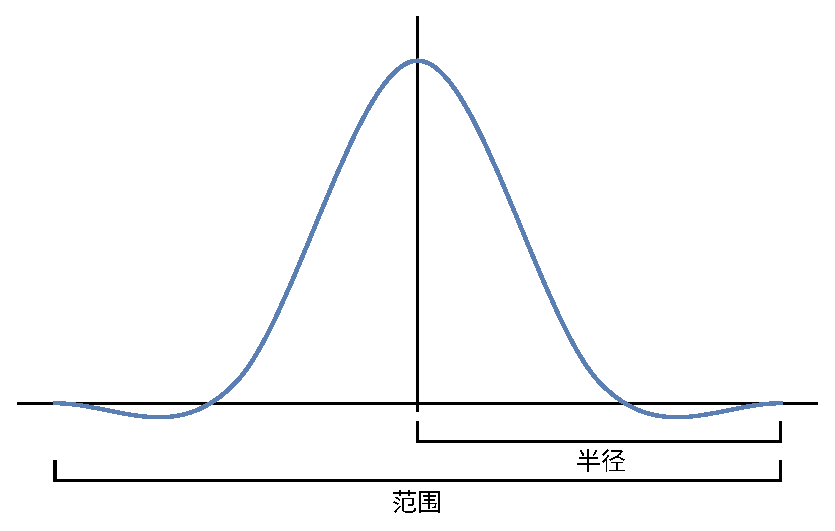
\includegraphics[width=0.6\linewidth]{chap07/filter-extent-radius.eps}
    \caption{pbrt中滤波器的范围是依据从原点到其截断点的半径来指定的。
        滤波器的支撑域是其整个非零范围,这里等于其半径的两倍。}
    \label{fig:7.40}
\end{figure}

所有滤波器中心都在原点$(0,0)$且定义了半径,超出半径时它们都取值为0;
该宽度也许在$x$和$y$方向是不同的。
构造函数接收半径值并和其倒数一块儿保存,以供滤波器实现使用。
滤波器在每个方向的整个范围(它的支撑域)是其相应半径值的两倍(\reffig{7.40})。
\begin{lstlisting}
`\initcode{Filter Interface}{=}\initnext{FilterInterface}`
`\refvar{Filter}{}`(const `\refvar{Vector2f}{}` &radius)
    : `\refvar[Filter::radius]{radius}{}`(radius),
      `\refvar[Filter::invRadius]{invRadius}{}`(`\refvar{Vector2f}{}`(1 / radius.x, 1 / radius.y)) { }
\end{lstlisting}
\begin{lstlisting}
`\initcode{Filter Public Data}{=}`
const `\refvar{Vector2f}{}` `\initvar[Filter::radius]{radius}{}`, `\initvar[Filter::invRadius]{invRadius}{}`;
\end{lstlisting}

\refvar{Filter}{}实现需要提供的唯一方法是\refvar[Filter::Evaluate]{Evaluate}{()}。
它接收一个给出了样本点相对于滤波器中心位置的2D点参数。
返回滤波器在该点的值。系统中别处的代码永远不会用滤波器范围外的点来调用滤波函数,
所以滤波器实现不需要检查这种情况。
\begin{lstlisting}
`\refcode{Filter Interface}{+=}\lastcode{FilterInterface}`
virtual `\refvar{Float}{}` `\initvar[Filter::Evaluate]{Evaluate}{}`(const `\refvar{Point2f}{}` &p) const = 0;
\end{lstlisting}

\subsubsection*{矩形滤波器}
图形学中最常用的滤波器之一是\keyindex{矩形滤波器}{box filter}{filter滤波器}
(且实际上当没有明确解决滤波和重建时,矩形滤波器就是\emph{事实上}的结果)。
